%===================================================================================================
%===================================================================================================
\section{Pipeline Parallelism}
\label{sec:pipeline-parallelism}
%===================================================================================================
%===================================================================================================

Suppose that we have a neural network which is represented as a composition of sequence of subnetworks. Let us denote the subnetworks by $f^1, \cdots, f^n$ with parameters $\theta^1, \cdots, \theta^n$ and let the full network be 
\[
    f = f^n \circ f^{n-1} \circ \cdots \circ f^1,
\]
parameterized by $\theta = (\theta^1, \cdots, \theta^n)$. For clarity, we call $f^j$ \emph{the $j$th partition of $f$} and assume that the parameters of partitions are mutually disjoint. 

When training the network, gradient-based methods such as stochastic gradient descent requires computing the outcome $f(x)$ of the network given a mini-batch $x$ of training data and the corresponding loss, and the gradient $g$ of the loss with respect to the network parameter $\theta$. Those two stages are called forward and backward pass, respectively. 

Since $f$ is sequentially composed, in forward pass $f(x)$ can be computed by letting $x^0 = x$ and sequentially applying the partitions as $x^j = f^j(x^{j-1})$ for $j=1,\cdots,L$. Furthermore, if $x$ consists of $m$ smaller batches $x_1, \cdots, x_m$ called \emph{micro-batches}, computing $f(x)$ dissolves into tasks $F_{i,j}$ where $x^0_i = x_i$ and 
\begin{equation}
\tag{$F_{i,j}$}
x_i^j \ot f^j(x_i^{j-1})
\end{equation}
for $i=1,\cdots,m$ and $j=1, \cdots, n$, assuming that $f$ does not involve any intra-batch computation. One prominent exception for this is batch normalization \cite{pmlr-v37-ioffe15}\footnote{Applying pipeline parallelism to a network with batch normalization is feasible while the computation is not identical anymore. Indeed, this discrepancy also exists in data-parallel training scheme and it may results in degradation of the result.}. The loss is obtained by aggregating $x_i^n = f(x_i)$ and evaluating the loss function on them.

In a similar fashion, backward pass is decomposed into tasks $B_{i,j}$ where $dx_i^{n}$ is the gradient of the loss with respect to $x_i^n$ and
\begin{equation}
\tag{$B_{i,j}$}
\begin{aligned}
dx_i^{j-1} &\ot \partial_x f^j (dx_i^{j}) \\
g_i^{j} &\ot \partial_{\theta^j} f^j (dx_i^j)
\end{aligned}
\end{equation}
for $i=1,\cdots,m$ and $j=1,\cdots,n$. Here
\[
    \partial_x f^j : v \mapsto v^T \cdot \left.\frac{d f^j}{d x}\right|_{x=x_i^{j-1}}
\]
is a function which does backward propagation (also known as vector-Jacobian product) through the partition $f^j$, and $\partial_{\theta^j} f^j$ is defined likewise. As a result, we get the gradient of the loss with respect to $\theta^j$ by summing $g_i^j$ over $i$'s.

Note that there are data dependencies between tasks. For example, $F_{i, j}$ requires $x_i^{j-1}$ which is only available after $F_{i, j-1}$, hence $F_{i, j-1}$ must be completed before starting $F_{i, j}$ and the same applies for $B_{i, j}$ and $B_{i, j+1}$. \autoref{fig:dependency} shows the full dependency graph in the case of $m=4$ and $n=3$.

\begin{figure*}
    \centering
    \hspace{0.02\textwidth}
    \begin{minipage}[c][340pt][t]{0.40\textwidth}
        \vspace*{\fill}
        \centering
        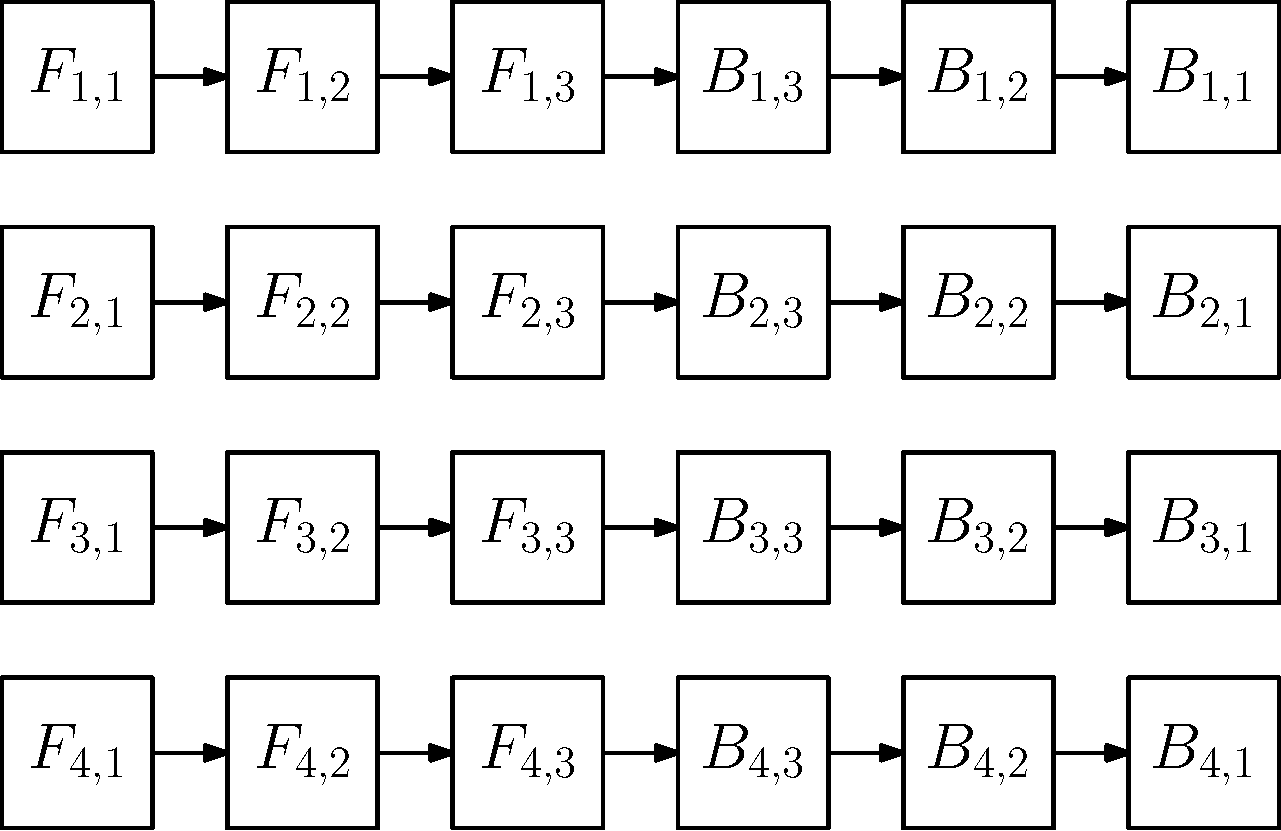
\includegraphics[width=0.95\textwidth]{figures/dependency.pdf}
        \caption{Minimal dependency graph for forward and backward pass.}
        \label{fig:dependency}\par\vfill
        \vspace{10pt}
        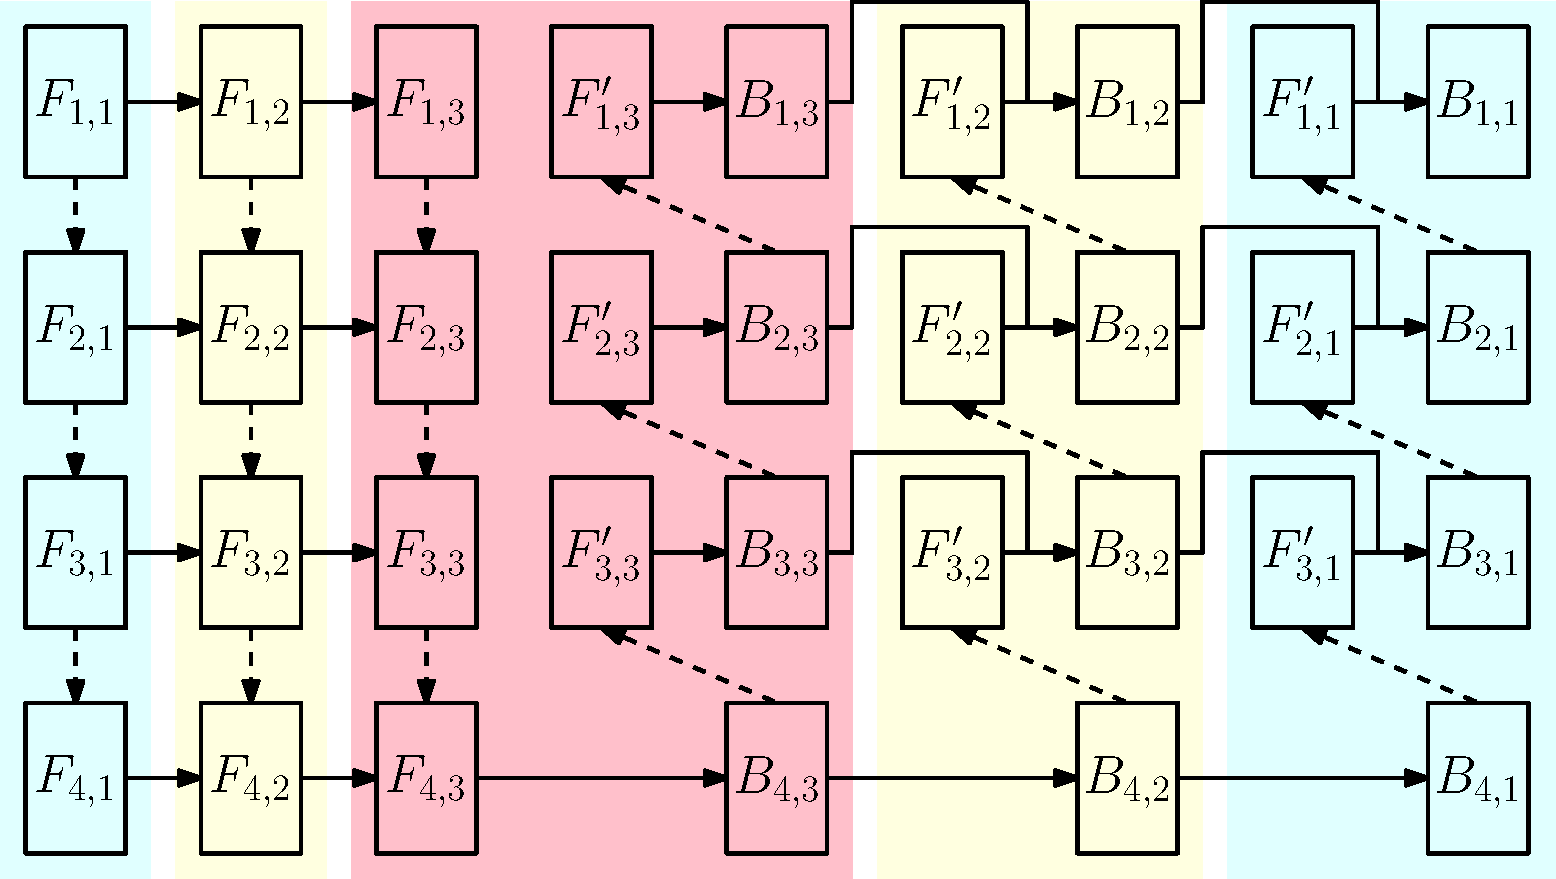
\includegraphics[width=\textwidth]{figures/pp-with-checkpointing.pdf}
        \caption{Dependency graph for pipeline parallelism with checkpointing. Colors denote the devices that tasks are computed in.}
        \label{fig:pp-with-checkpointing}
    \end{minipage}
    \hspace{0.03\textwidth}
    \begin{minipage}[c][292pt][t]{0.53\textwidth}
        \vspace*{\fill}
        \centering
        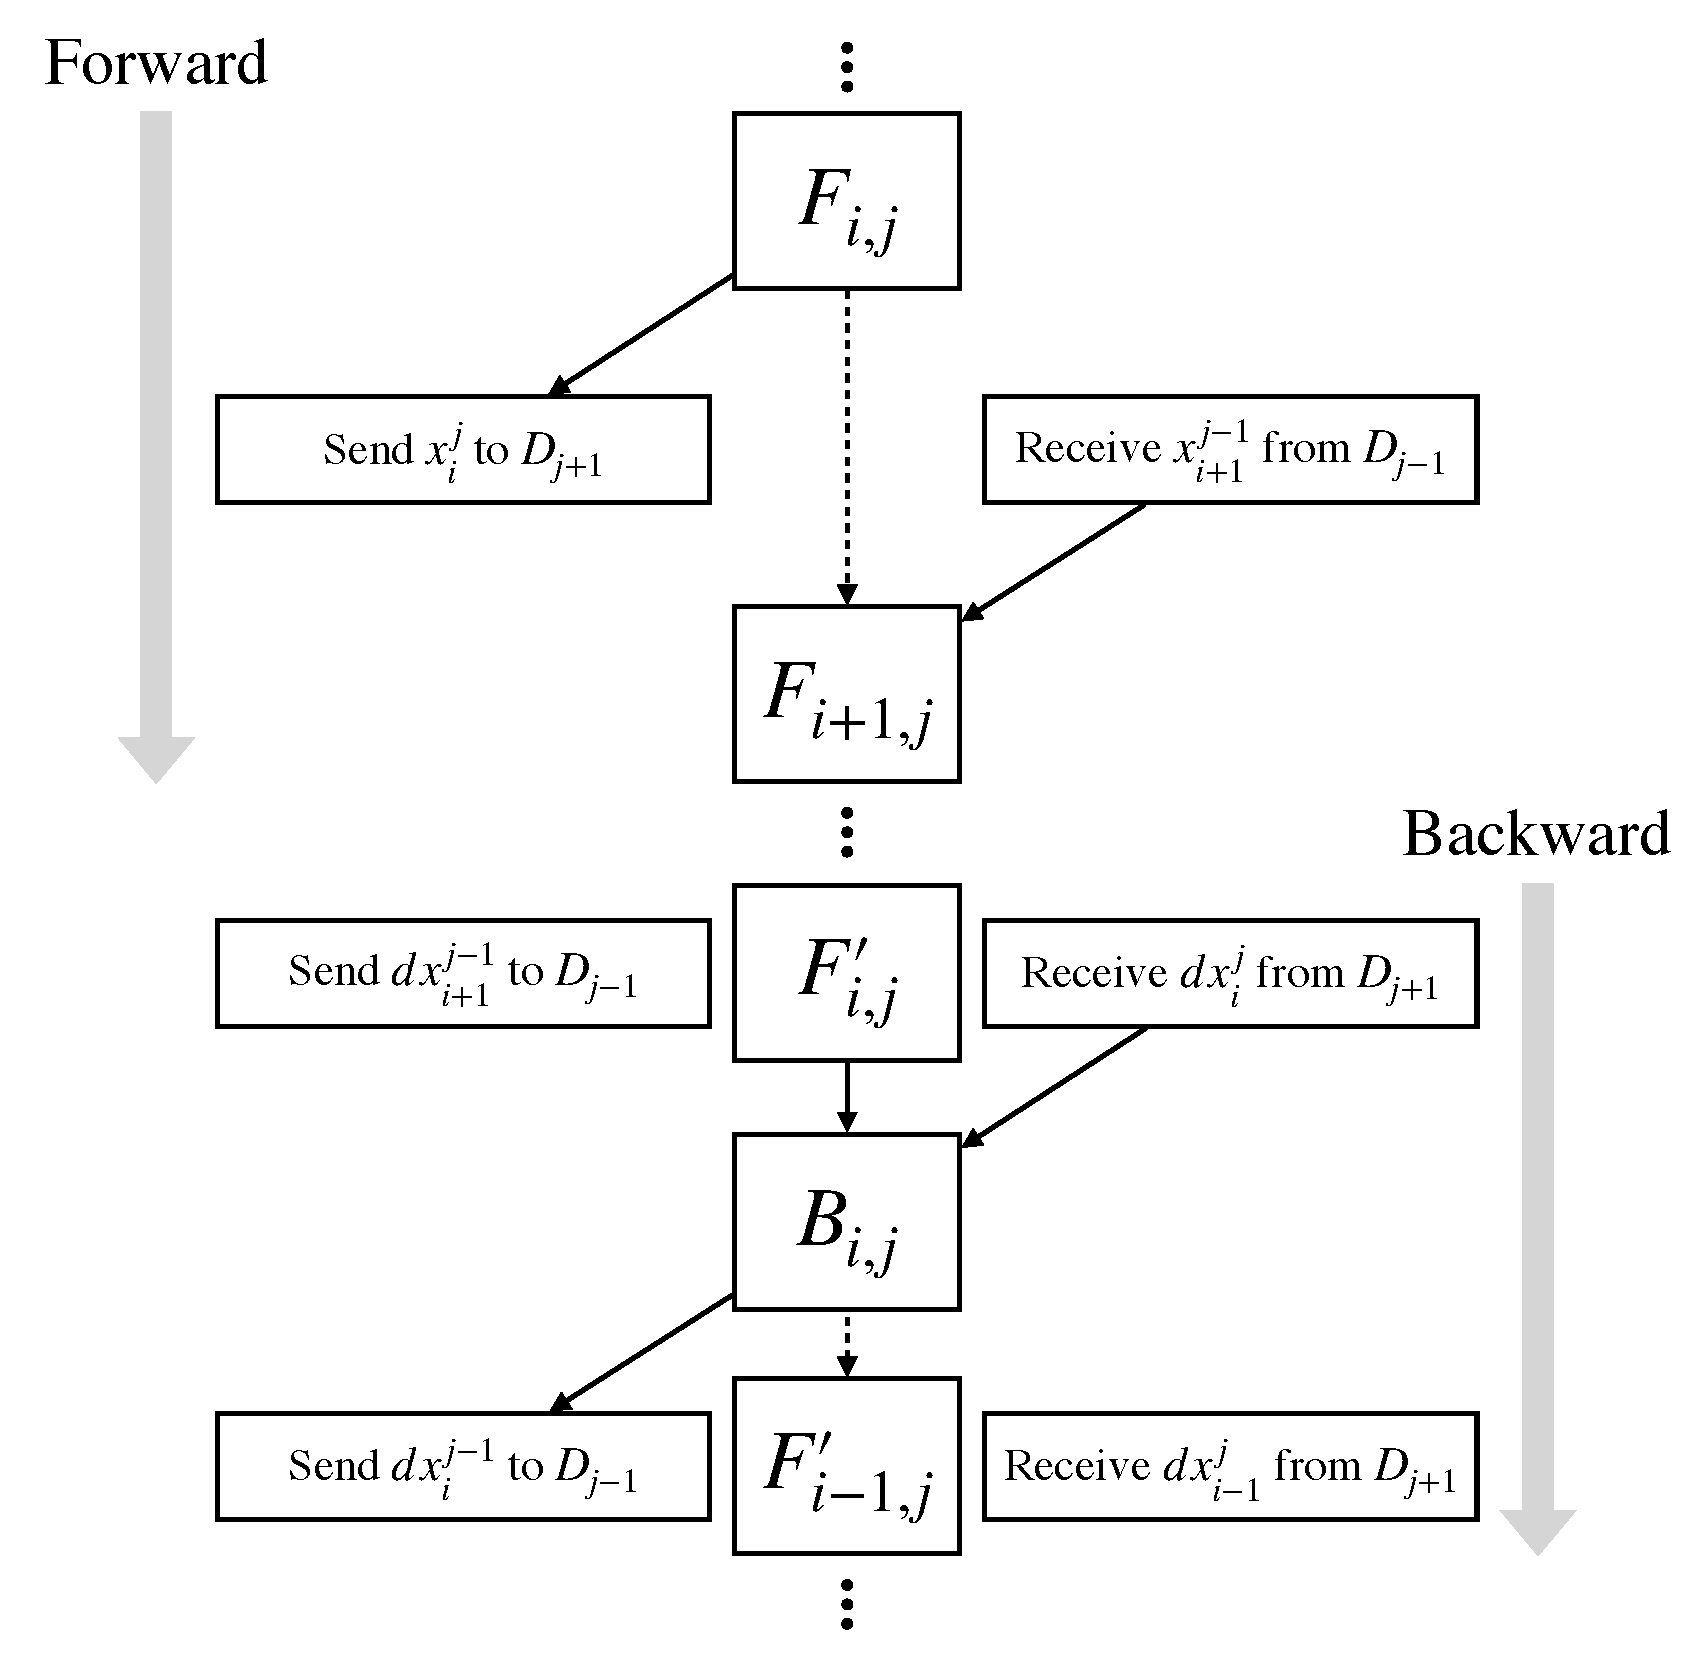
\includegraphics[width=\textwidth]{figures/kernel-order.pdf}
        \caption{The execution order that $j$th device must follow.}
        \label{fig:kernel-order}
    \end{minipage}
\end{figure*}

Given the set of tasks $\{F_{i, j}\}$ and $\{B_{i, j}\}$ and a pool of devices which can work in parallel, different parallelization strategies have their own rule to assign tasks to devices. Each device computes one or more assigned tasks as soon as the dependencies are resolved. In the setting above, all dependencies are among the tasks with the same micro-batch index $i$. Hence, one can effectively parallelize the tasks by assigning tasks with different micro-batch indices to different devices --- which is data parallelism.

\subsection{Dependency Graph of GPipe}
\label{subsec:gpipe-dependency}

Pipeline parallelism's strategy is to assign tasks with respect to the partition index $j$ so that $j$th partition entirely lies in the $j$th device. In addition to this, it is enforced that $F_{i, j}$ must be completed before executing $F_{i+1, j}$ and $B_{i, j}$ must be completed before executing $B_{i-1, j}$. 

In addition to the micro-batch pipelining, GPipe \cite{huang2019gpipe} further reduces the memory requirement by utilizing gradient checkpointing for each $B_{i, j}$. Since $j$th device executes $B_{i,j}$ one at a time, only the activation maps obtained from $F_{i,j}$ are needed to complete $B_{i,j}$. By recomputing the forward pass $F_{i,j}$ right before executing $B_{i,j}$, memory consumption is reduced by a factor of $m$. Moreover, the re-computation can take place while the device is waiting for $B_{i,j+1}$ being done. This is summarized in \autoref{fig:pp-with-checkpointing}, where dashed arrows denotes the execution order between independent tasks induced by the micro-batch order, and $F_{i, j}'$ denotes the re-computation of $F_{i,j}$. 


We remark that re-computations for the last micro-batch, \emph{i.e.}, $F_{m, j}'$ for $j=1,\cdots,n$ are unnecessary. This is because that on $j$th device the last task in the forward pass is $F_{m, j}$, so discarding intermediate activations of it in forward pass and re-computing them in the beginning of backward pass has no effect of reducing memory, only slowing down the pipeline. For this reason, $F_{m, j}'$ is omitted from the graph.

\subsection{Device-wise Execution Order}
\label{subsec:timeline}

To summarize, in pipeline parallelism (with checkpointing) each device is assigned with a set of tasks with the prescribed order. Each device will execute the given tasks one-by-one as soon as cross-device dependencies are met. However, there is a missing component in this picture --- data tranfer between the devices. For illustration, the full execution order that device $j$ must follow is shown in \autoref{fig:kernel-order}. Here data transfer operations are explicitly denoted as `receive' and `send' for emphasis.

% \begin{center}
% \fbox{
% \begin{minipage}[c]{0.4\textwidth}
% \begin{tabular}{l}
% $\vdots$
% \\ receive $x_{i}^{j-1}$ from device $j-1$.
% \\ execute $F_{i,j}$.
% \\ send $x_i^j$ to device $j+1$.
% \\ receive $x_{i+1}^{j-1}$ from device $j-1$.
% \\ [-0.8ex] $\vdots$
% \\ execute $F_{i,j}'$.
% \\ receive $dx_i^{j}$ from device $j+1$.
% \\ execute $B_{i,j}$.
% \\ send $dx_i^{j-1}$ to device $j-1$.
% \\ execute $F_{i-1, j}'$.
% \\ [-0.8ex] $\vdots$
% \end{tabular}
% \vspace{0.8ex}
% \end{minipage}
% }
% \end{center}
